\begin{tikzpicture}
\node[inner sep=0,anchor=south west] (im) at (0,0) {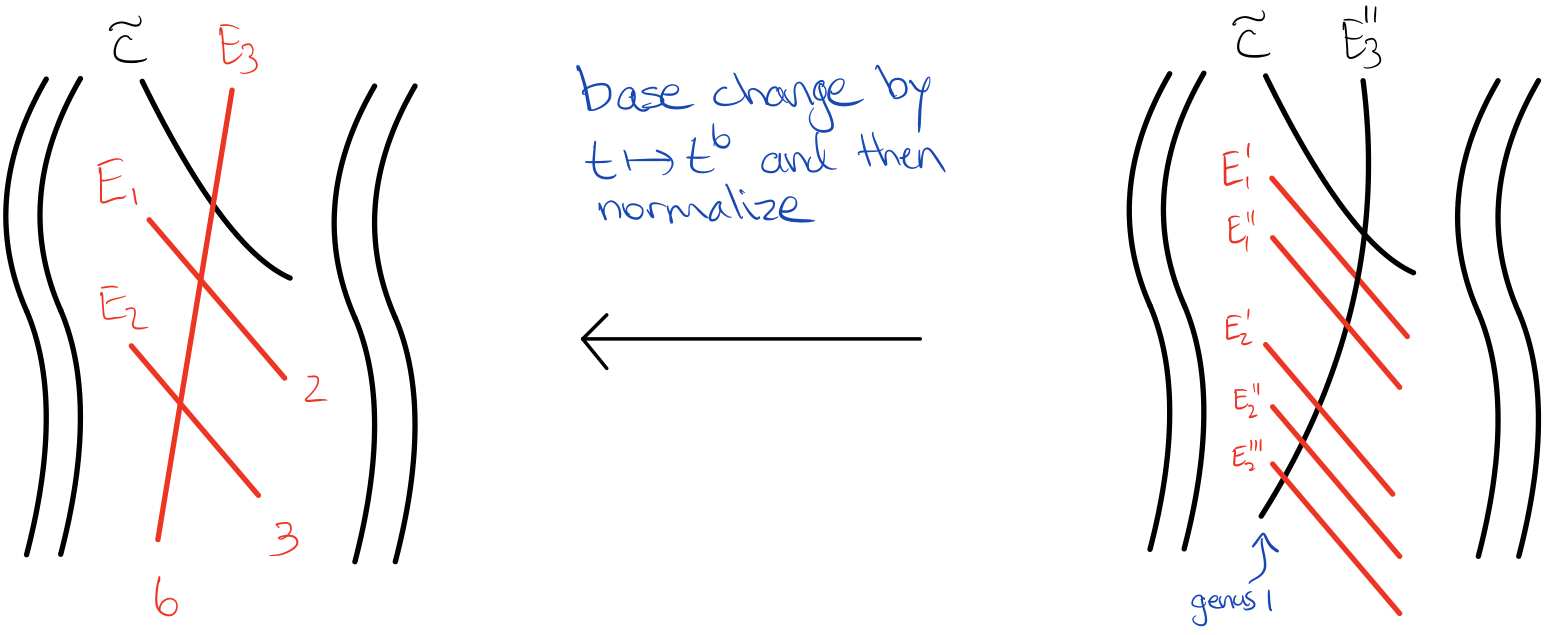
\includegraphics[width=.86\textwidth]{figures/reduction-step4.png}};
\begin{scope}[x={(im.south east)},y={(im.north west)}]
\fill[white] (0.36,0.63) rectangle (0.62,0.91);
\fill[white] (0.75,0.015) rectangle (0.83,0.1);
\node[fill=white,inner sep=1pt,font=\scriptsize,text=blue] at (0.5,0.83) {沿 $t\mapsto t^6$};
\node[fill=white,inner sep=1pt,font=\scriptsize,text=blue] at (0.5,0.71) {基变换并正规化};
\node[fill=white,inner sep=1pt,font=\scriptsize,text=blue] at (0.8,0.035) {亏格 $1$};
\end{scope}\end{tikzpicture}
